\documentclass{article}

\usepackage{amsmath,amssymb,amsthm,graphicx}

\setlength{\oddsidemargin}{0.25 in}
\setlength{\evensidemargin}{-0.25 in}
\setlength{\topmargin}{-0.6 in}
\setlength{\textwidth}{6.5 in}
\setlength{\textheight}{8.5 in}
\setlength{\headsep}{0.75 in}
\setlength{\parindent}{0 in}
\setlength{\parskip}{0.1 in}

\newtheorem{theorem}{Theorem}
\newtheorem{corollary}{Corollary}
\newtheorem{proposition}{Proposition}
\newtheorem*{remark}{Remark}
\theoremstyle{definition}
\newtheorem{example}{Example}
\newtheorem{definition}{Definition}

\newcommand{\lecture}[4]{
   \pagestyle{myheadings}
   \thispagestyle{plain}
   \newpage
%   \setcounter{lecnum}{#1}
   \setcounter{page}{1}
   \noindent
   \begin{center}
   \framebox{
      \vbox{\vspace{2mm}
    \hbox to 6.58in { {\bf CSC~565: Graph Theory
                        \hfill North Carolina State University} }
    \hbox to 6.58in { {\bf Fall 2019
                        \hfill Computer Science} }
       \vspace{4mm}
       \hbox to 6.28in { {\Large \hfill Lecture #1: #2  \hfill} }
       \vspace{2mm}
       \hbox to 6.28in { {\it Lecturer: {\it Don Sheehy {\tt <drsheehy@ncsu.edu>}} \hfill Scribe: #4} }
      \vspace{2mm}}
   }
   \end{center}
   \markboth{Lecture #1: #2}{Lecture #1: #2}
   \vspace*{4mm}
}


\begin{document}


%FILL IN THE RIGHT INFO.
%\lecture{**LECTURE-NUMBER**}{**DATE**}{**SCRIBE**}
\lecture{1}{Aug 21, 2019}{ Lauren Alvarez }
  % \title{Lecture 1}
  % \author{Scribed by: }
  % \maketitle

\section{Pre-class logistics}
\section{The Basics}
Graphs are the most important abstraction in computation (after numbers and sets)
\begin{itemize}
    \item They describe binary relations (i.e. sets of pairs of things)
    
    \item As the name implies, we often draw graphs
     \begin{figure}[h]
    \centering
    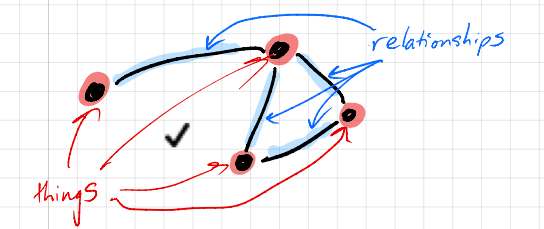
\includegraphics[width=0.5\textwidth]{images/graphbasics.png}
    \caption{The drawing is not the graph. It's only a picture.}
    \label{fig:}
\end{figure}
    \item Graphs are everywhere
       \begin{itemize}
       \item Circuits
       \item Networks
       \item Roadmaps
       \item Data Structures
       \item ... and other less obvious settings as well
       \end{itemize}
     
\end{itemize}

\section{Introduction: What is graph?}
When we talk about graphs, we could first start with some of the basic building component of it:
\begin{itemize}
    \item Number
     \begin{center}
        1, 2
     \end{center}
    \item Set
     \begin{center}
      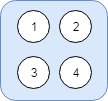
\includegraphics{images/set.png}
     \end{center}
    \item Graph
     \begin{center}
      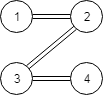
\includegraphics{images/graph.png}
     \end{center}
\end{itemize}

\section{Definitions}
\begin{itemize}
    \item A \textbf{graph} is a pair (V,E) where V is any set and E is a set of 2-elements subset (``unordered pairs") of V
    \item The set V is called the \textbf{vertex set} and its elements are called \textbf{vertices}
    \item The set E is called the \textbf{edge set} and its elements are called \textbf{edges}
    \item We often write \textit{G = (V,E)} to assign a name (G) to a graph (V,E)
    \item We may also write \textit{V(G)} and \textit{E(G)} to refer to the vertex and edge sets of some given graph G
\end{itemize}

\subsection{Examples}
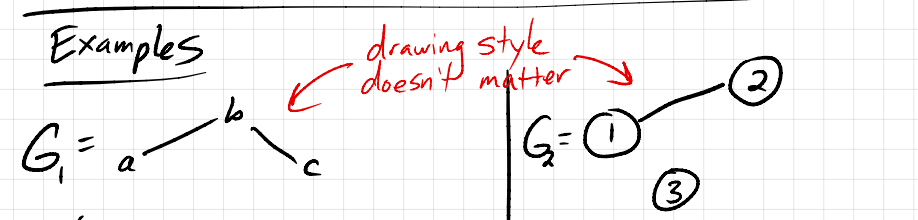
\includegraphics[width=0.75\textwidth]{images/examples.png}

\textbf{$G_1$:}

$V(G_1) = \{a,b,c\}$

$E(G_1) = \{\{a,b\},\{b,c\}\}$

\textbf{$G_2$:}

$V(G_2) = \{1,2,3\}$

$E(G_2) = \{\{1,2\}\}$

\textit{Notation: It's easier to write (a,b) instead of \{a,b\}. In this case, it's assumed (a,b) = (b,a). }

\begin{itemize}
    \item Two vertices u,v are \textbf{adjacent} if $(u,v) \epsilon E$
    \item An edge e and a vertex v are \textbf{incident} if $v \epsilon e$ (i.e. $e = (u,v)$ for some $u \epsilon V$
    \item The number of edges incident to a vertex v is called a degree of v, and is written \itemit{deg(v)}
\end{itemize}
\subsection{Exercise}
 Prove $$\sum_{v \epsilon V} deg(v) = 2|E|$$ for any graph (V,E)
 
 
 \section{Graph Questions}
 \begin{enumerate}
  \item Is it connected? (i.e. is it all one piece)
  \item Does the graph have any cycles?
  \item What is the shortest path form one vertex to another?
  \item Can we assign a small number of colors to the vertices so that no two adjacent vertices have the same color?
  \item Can we draw the graph so that no two edges cross?
  \item Is one graph ``equal" to another (allowing the vertices to be relabelled)
  \item Does one graph contain another graph (or its equivalent)?
  \item How quickly will a random walk on a graph mix?
  \item How many spanning trees (minimally connected subgraphs using all the vertices) does a graph contain?
\end{enumerate}

\section{Different Perspective on Graphs}
Combinatorics, Computation, Geometry, Topology, Algebra. As much as possible, we will try to represent these different perspectives as \textbf{categories} and our change of perspective as \textbf{functions}. I will tell you what these words mean.

\subsection{Sets and Functions}
\textit{This should all be review I will use all these concepts, definitions, and notation will reckless abandonment.}
The definition of a graph depends on the notion of a set. 

You should know:
\begin{enumerate}
    \item \underline{What is a set?} 
    
    Elements, Membership, Empty Set ($\O$), Cardinality
    \item \underline{Set Relations and Elements}
    
    $a \epsilon S$ ``a is in S" or ``a is an element of S"
    
    $A \subset B$, $A \subseteq B$, $A = B$
    \item \underline{Set Operations}
    
    Union: $A \cup B$ 
    
    Intersection: $A \cap B$
    
    Difference: $A \setminus B$
    
    Complement: $\hat{A}$
    
    Cartesian Product: $A X B$
    
    $\bigcup\limits_{i = 1}^{n} A_i$ ,  $\bigcap\limits_{i = 1}^{n} A_i$
    \item \underline{Notation}
    $\{1,2,3\}$
    
    (Sub) Set Builder: $\{x \epsilon \mathbb{R}| x \geq 2\}$
    
    Predicate: $x \geq 2$
    \item \underline{Functions}
    $f: A \Rightarrow B$
    
    domain, range, injective, surjective, bijective, inverse, preimage, composition

\end{enumerate}
\subsection{The Category of Sets}
\begin{itemize}
\item Set fuctions: $f: A \Rightarrow B$ or $A \xrightarrow{f}B$

A is the \textbf{domain} or \textbf{source}

B is the \textbf{range} or \textbf{target}

\item Functions can be \textbf{composed}

$A \xrightarrow{f}B\xrightarrow{g}C$

$A \xrightarrow{g\circ f}C$

$x \epsilon A: (g \circ f)(x) = g(f(x)) \epsilon C$

\item \textbf{Inclusion} (as a function)

If $a \subseteq B$ there exists a unique injection $f: A \Rightarrow B$ such that for all $x \epsilon A: f(x) = x$

\item Identity Functions

For any set A there is a unique fucntion $id_A: A \Rightarrow A$ such that for all $x\epsilon A \quad id_A(x) = x$

\item Let A,B be sets and $f: A \Rightarrow B$
\subitem \textbf{Image}
 $im f = \{f(x): x \epsilon A\} \subseteq B$
 \item Let $S \subseteq A$
 \subitem \textbf{Restriction}
 $f_{\setminus S}: S\Rightarrow B$
 $f_{\setminus S}(x) = f(x)$ (for all $x \epsilon S$)
 \subitem \textbf{Image of a set}
 $f(s) = imf_{\setminus S} = \{f(x): x\epsilon S\}$
 
 (\textit{Note: This is an abuse of notation and I'm not sorry.})
 \subitem \textbf{Preimage}
 $ T \subseteq B$
 $f^{-1}(T) = \{x \epsilon A: f(x) \epsilon T \}$ 
 
 (\textit{Another abuse of notation. $f^{-1}$ could also be an inverse.})
 
 \subitem \textbf{Inverse}
 If f is bijective then there is a unique function $f^{-1}: B \Rightarrow A$ such that $ f\circ f^{-1} = id_B$ and $f^{-1} \circ f = id_A$
\end{itemize}


\end{document}
